\phantomsection

\chapter{Resultados}\label{ch:capitulo_resultados}

Este capítulo apresenta os sinais e valores obtidos no experimento realizado no dispositivo de flexão.
Os tópicos aqui analisados apresentam a comparação dos resultados obtidos pelo experimento realizado pelo autor com os valores obtidos pelo
estudo de caso feito por Minela (2017).

O objetivo primário da comparação dos resultados é o de se obter dados descritivos de performance do dispositivo desenvolvido em relação a um sistema de medição industrial
homologado, no final do capítulo são indicados as situações de melhor performance do protótipo.

\section{Sinais obtidos}

Os sinais captados pelo sistema de medição desenvolvido seguem um formato trapezoidal, onde as zonas iniciais e finais representam os momentos em que a viga não se encontrava
sob a aplicação da carga, e a zona intermediária representa a total aplicação da carga no dispositivo.

\subsection{Sinais de calibração}

A primeira etapa da utilização do dispositivo é definir os sinais de calibração, para isso é obtido as respostas de leitura do amplificador de sinal para a aplicação das cargas
de 0,138kg e 1,04kg, que representavam o menor e o maior peso disponível para o experimento, sem considerar as combinações.

Foi obtido o valor médio de 190 bits na zona superior do sinal trapezoidal na aplicação da massa de 0,138kg, como mostradado na \autoref{fig:410}.
Para a aplicação da massa de 1.04kg foi obtido o valor de 612 bits, mostrado na \autoref{fig:420}.

\begin{figure}[H]
	\caption{\label{fig:410} Sinal obtido pela aplicação da carga de 0,138kg no dispositivo}
	\begin{center}
		\includegraphics[width=350]{pictures/signals/cal_signal_1.png}
	\end{center}
	\fonte{O autor 2022}
\end{figure}

\begin{figure}[H]
	\caption{\label{fig:420} Sinal obtido pela aplicação da carga de 1,04kg no dispositivo}
	\begin{center}
		\includegraphics[width=350]{pictures/signals/cal_signal_2.png}
	\end{center}
	\fonte{O autor 2022}
\end{figure}

Uma vez obtidos os valores em bits para cada ponto de calibração e conhecidos os seus valores de deformação teóricos, é calculado os fatores $ a $ e $ b $ da função de interpolação
linear que converte valores obtidos pelo amplificador de sinal em bits para valores equivalentes de deformação no extensômetro.
O valor do fator a encontrado foi de $ 2.8881 {\mu}m/bit $ e o de b foi de $ -363.4311 {\mu}m $.

Uma vez definidos os parâmetros de calibração são feitos os experimentos aplicando a carga de cada peso no dispositivo de flexão.
Alguns dos sinais obtidos e uma discussão geral sobre eles são discutidos nas seções a seguir.

\subsection{Sinais calibrados obtidos}

O experimento é realizado obtendo os sinais calibrados obtidos pelo dispositivo na aplicação de cada uma das massas disponíveis e pela aplicação de combinações entre essas massas,
os valores de cargas aplicadas para a realização dos experimentos são mostradas na \autoref{tab:Cargasaplicadas}.

\begin{table}[H]
    \caption{Cargas aplicadas para os experimentos}
    \label{tab:Cargasaplicadas}
    \centering
    \resizebox{350}{!}{%
        \begin{tabular}{ l c r } \toprule
			Pesos aplicados & {Massa aplicada (Considerando fuso e porca)} \\
			Peso 1 & 138.42 \\
			Peso 2 & 250.07 \\
			Peso 3 & 1048.82 \\
			Peso a & 549.35 \\
			Pesos 1 e 2 & 336.8 \\
			Pesos 1 e a & 636.08 \\
			Pesos 2 e a & 747.73 \\
			Pesos 1, 2 e a & 834.46 \\
			Pesos 3 e 1 & 1135.55 \\
			Pesos 3 e 2 & 1247.2 \\
			Pesos 3, 2 e 1 & 1333.93 \\
            \bottomrule
        \end{tabular}}
\fonte{O autor 2022}
\end{table}

O primeiro peso aplicado é o de menor massa disponível, que ja tinha sido previamente utilizada para utilização na calibração do dispositivo,
o sinal obtido é mostrado na \autoref{fig:4102}, o valor de deformação obtido foi de $ 182.42 {\mu}m $.

\begin{figure}[H]
	\caption{\label{fig:4102} Sinal obtido da aplicação de 0,138 kg de carga aplicada no dispositivo}
	\begin{center}
		\includegraphics[width=350]{pictures/signals/w1.png}
	\end{center}
	\fonte{O autor 2022}
\end{figure}

O sinal equivalente obtido por Minela (2017) é mostrado na \autoref{fig:4102_m}.

\begin{figure}[H]
	\caption{\label{fig:4102_m} Sinal obtido da aplicação da massa ded 0,163 kg de carga aplicada no dispositivo}
	\begin{center}
		\includegraphics[width=350]{pictures/signals/wp1.png}
	\end{center}
	\fonte{\autocite{Minela2017}}
\end{figure}

Uma comparação direta de valor não pode ser feita considerando os dois sinais, uma vez que as massas aplicadas não foram as mesmas, porém,
pode-se notar que o efeito dos ruídos no dispositivo desenvolvido é consideravelmente menor do que os obtidos pelo dipositivo utilizado em Minela (2017).
A atuação dos filtros de passa-altas do módulo de conversão de sinal utilizado no dispositivo desenvolvido pode ser o principal motivo pelos quais os ruídos em
todos os resultados obtidos pela utilização do protótipo desenvolvido se mostraram de baixas amplitudes.

O sinal obtido pela aplicação do de 1,04kg é mostrado na \autoref{fig:4109}, o valor de deformação obtido foi de $ 1421.41 {\mu}m $.

\begin{figure}[H]
	\caption{\label{fig:4109} Sinal obtido da aplicação de 1,040 kg de carga aplicada no dispositivo}
	\begin{center}
		\includegraphics[width=350]{pictures/signals/w8.png}
	\end{center}
	\fonte{O autor 2022}
\end{figure}

O sinal equivalente obtido por Minela (2017) é mostrado na \autoref{fig:4109_m}

\begin{figure}[H]
	\caption{\label{fig:4109_m} Sinal obtido da aplicação da massa ded 0,163 kg de carga aplicada no dispositivo}
	\begin{center}
		\includegraphics[width=350]{pictures/signals/wp3.png}
	\end{center}
	\fonte{\autocite{Minela2017}}
\end{figure}

Assim como no primeiro sinal, nota-se que os sinais são semelhantes, com a excessão dos ruídos, que são mais impactantes com 
a utilização do dispositivo utilizado por Minela (2017) do que com a utilização do protótipo desenvolvido.

Os sinais obtidos para carga utilizada no experimento podem ser encontrados no \autoref{ch:sinais-obtidos}.

Utilizando a \autoref{eq:Eq_201} pode-se obter analiticamente valores de deformação esperados para cada situação de carga do experimento.
O valor de módulo de elasticidade utilizado no modelo analítico foi de $ 85.19 GPa $, que é um valor obtido experimentalmente no trabalho de Minela (2017)
para o mesmo dispositivo utilizado.
A \autoref{tab:ResultadosDeformacao} mostra os resultados de valores de deformação obtidos para cada experimento, os valores de deformação esperados
calculados e os valores de erro de cada resultado obtido em relação ao teórico.

\begin{table}[H]
    \caption{Cargas aplicadas para os experimentos}
    \label{tab:ResultadosDeformacao}
    \centering
    \resizebox{350}{!}{%
        \begin{tabular}{ l c r } \toprule

            \bottomrule
        \end{tabular}}
\fonte{O autor 2022}
\end{table}





%A \autoref{fig:4010} mostra os valores nominais de deformação para cada leitura da zona intermediária de cada sinal para cada combinação de cargas
%realizadas na execução do experimento, assim como o valor médio das amostras para cada combinação e o desvio padrão dos dados na zona intermediária
%de cada sinal como avaliação dos ruídos presentes.
%
%\begin{figure}[htb]
%	\caption{\label{fig:4010} Amostras e valores médios obtidos}
%	\begin{center}
%		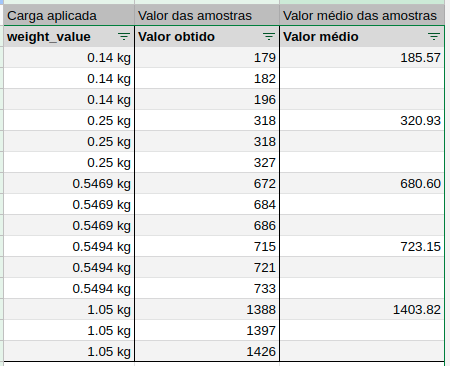
\includegraphics[width=\textwidth]{pictures/val_func_cal.png}
%	\end{center}
%	\fonte{O autor 2022}}
%\end{figure}

%Os Valores de carga compensados pelo problema da porca e do peso não encontrados conforme indicado na \autoref{}, junto com a comparação dos resultados obtidos por
%\autocite{Minela2017} são mostrados na \autoref{}.

%\section{Comparação final}
%
%A \autoref{} compara os principais resultados obtidos pelo experimento desenvolvido pelo autor com os resultados obtidos pelo trabalho de \autocite{Minela2017}.


%% TODO IMAGENS DE CARGAS


